\documentclass{article}
\usepackage[utf8]{inputenc}
\usepackage{listings}
\usepackage{multimedia} % to embed movies in the PDF file
\usepackage{graphicx}
\usepackage{comment}
\usepackage[english]{babel}
\usepackage{amsmath}
\usepackage{amsfonts}
\usepackage{subfigure}
\usepackage{wrapfig}
\usepackage{multirow}
\usepackage{tikz}
\usepackage{verbatim}

\newtheorem{theorem}{Theorem}[section]
\newtheorem{lemma}[theorem]{Lemma}
\newtheorem{corollary}[theorem]{Corollary}
%\newtheorem{algorithm}[theorem]{Algorithm}
\newtheorem{remark}[theorem]{Remark}
\newenvironment{proof}{\noindent {\bf Proof:} }{\hfill $\Box$ \\[2ex] }
\newenvironment{keywords}{\begin{quote} {\bf Key words} }
                         {\end{quote} }
\newenvironment{AMS}{\begin{quote} {\bf AMS subject classifications} }
                         {\end{quote} }


\newcommand{\eref}[1]{\mbox{\rm(\ref{#1})}}
\newcommand{\tref}[1]{\mbox{\rm\ref{#1}}}
\newcommand{\set}[2]{\left\{ #1 \; : \; #2 \right\} }
\newcommand{\deq}{\raisebox{0pt}[1ex][0pt]{$\stackrel{\scriptscriptstyle{\rm def}}{{}={}}$}}

\newcommand {\DS} {\displaystyle}

\newcommand{\real}{\mathbb{R}}
\newcommand{\compl}{\mathbb{C}}



\newcommand {\half} {\mbox{$\frac{1}{2}$}}
\newcommand{\force}{{\mathbf{f}}}
\newcommand{\strain}{{\boldsymbol{\varepsilon}}}
\newcommand{\stress}{{\boldsymbol{\sigma}}}
\renewcommand{\div}{{\boldsymbol{\nabla}}}

\newcommand {\cA} {{\cal A}}
\newcommand {\cB} {{\cal B}}
\newcommand {\cC} {{\cal C}}
\newcommand {\cD} {{\cal D}}
\newcommand {\cE} {{\cal E}}
\newcommand {\cL} {{\cal L}}
\newcommand {\cP} {{\cal P}}
\newcommand {\cQ} {{\cal Q}}
\newcommand {\cR} {{\cal R}}
\newcommand {\cV} {{\cal V}}
\newcommand {\cW} {{\cal W}}
\newcommand {\CH} {{\cal H}}
\newcommand {\CS} {{\cal S}}


\newcommand{\bzero}{\mathbf{0}}
\newcommand{\ba}{\mathbf{a}}
\newcommand{\bb}{\mathbf{b}}
\newcommand{\bc}{\mathbf{c}}
\newcommand{\bd}{\mathbf{d}}
\newcommand{\be}{\mathbf{e}}
\newcommand{\bff}{\mathbf{f}}
\newcommand{\bg}{\mathbf{g}}
\newcommand{\bh}{\mathbf{h}}
\newcommand{\bn}{\mathbf{n}}
\newcommand{\bp}{\mathbf{p}}
\newcommand{\bq}{\mathbf{q}}
\newcommand{\br}{\mathbf{r}}
\newcommand{\bs}{\mathbf{s}}
\newcommand{\bt}{\mathbf{t}}
\newcommand{\bu}{\mathbf{u}}
\newcommand{\bv}{\mathbf{v}}
\newcommand{\bw}{\mathbf{w}}
\newcommand{\bx}{\mathbf{x}}
\newcommand{\by}{\mathbf{y}}
\newcommand{\bz}{\mathbf{z}}
\newcommand{\bA}{\mathbf{A}}
\newcommand{\bB}{\mathbf{B}}
\newcommand{\bC}{\mathbf{C}}
\newcommand{\bD}{\mathbf{D}}
\newcommand{\bE}{\mathbf{E}}
\newcommand{\bF}{\mathbf{F}}
\newcommand{\bG}{\mathbf{G}}
\newcommand{\bH}{\mathbf{H}}
\newcommand{\bI}{\mathbf{I}}
\newcommand{\bJ}{\mathbf{J}}
\newcommand{\bK}{\mathbf{K}}
\newcommand{\bL}{\mathbf{L}}
\newcommand{\bM}{\mathbf{M}}
\newcommand{\bN}{\mathbf{N}}
\newcommand{\bO}{\mathbf{O}}
\newcommand{\bP}{\mathbf{P}}
\newcommand{\bQ}{\mathbf{Q}}
\newcommand{\bR}{\mathbf{R}}
\newcommand{\bS}{\mathbf{S}}
\newcommand{\bU}{\mathbf{U}}
\newcommand{\bV}{\mathbf{V}}
\newcommand{\bW}{\mathbf{W}}
\newcommand{\bX}{\mathbf{X}}
\newcommand{\bY}{\mathbf{Y}}
\newcommand{\bZ}{\mathbf{Z}}

\newcommand{\cO}{ {\cal O} }
\newcommand{\CT}{ {\cal T} }
\newcommand{\IL}{{\mathbb L}}
\newcommand{\sIL}{{{{\mathbb L}_s}}}
\newcommand{\bOmega}{{\boldsymbol{\Omega}}}
\newcommand{\bPsi}{{\boldsymbol{\Psi}}}

\newcommand{\bgamma}{{\boldsymbol{\gamma}}}
\newcommand{\bmu}{{\boldsymbol{\mu}}}
\newcommand{\blambda}{{\boldsymbol{\lambda}}}
\newcommand{\bLambda}{{\boldsymbol{\Lambda}}}
\newcommand{\bpi}{{\boldsymbol{\pi}}}
\newcommand{\bPi}{{\boldsymbol{\Pi}}}
\newcommand{\bphi}{{\boldsymbol{\phi}}}
\newcommand{\bPhi}{{\boldsymbol{\Phi}}}
\newcommand{\bpsi}{{\boldsymbol{\psi}}}
\newcommand{\btheta}{{\boldsymbol{\theta}}}
\newcommand{\bTheta}{{\boldsymbol{\Theta}}}
\newcommand{\bSigma}{{\boldsymbol{\Sigma}}}
\newcommand{\sump}{\sideset{}{^{'}}\sum} 
\DeclareMathOperator*{\Res}{Res}
\DeclareMathOperator{\OO}{O}
\DeclareMathOperator{\oo}{o}
\DeclareMathOperator{\erfc}{erfc}
\def\Xint#1{\mathchoice
   {\XXint\displaystyle\textstyle{#1}}%
   {\XXint\textstyle\scriptstyle{#1}}%
   {\XXint\scriptstyle\scriptscriptstyle{#1}}%
   {\XXint\scriptscriptstyle\scriptscriptstyle{#1}}%
   \!\int}
\def\XXint#1#2#3{{\setbox0=\hbox{$#1{#2#3}{\int}$}
     \vcenter{\hbox{$#2#3$}}\kern-.5\wd0}}
\def\ddashint{\Xint=}
\def\pvint{\Xint-}




\DeclareMathOperator\sign{sign}

\title{AMATH 570 Homework 2}
\author{Cade Ballew}
\date{October 22, 2021}

\begin{document}

\maketitle

\section{Problem 1 (Exercise 3.6)}
If we wish to spectrally differentiate two distinct real discrete functions $v$ and $w$ at once by the same two
complex FFTs, we define a new complex-valued function $u=v+iw$ and spectrally differentiate. Because $v$ and $w$ are both real, its derivative will be $u'=v'+iw'$, so we can just take the real and imaginary parts of the result of spectrally differentiating $u$ which would be the results of spectrally differentiating $v$ and $w$, respectively.\\
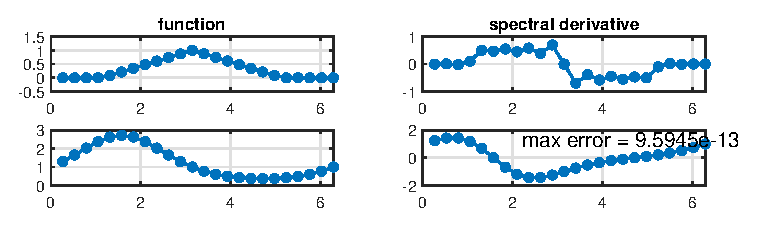
\includegraphics[]{prob3-6.eps}
\\The above figure is produced by modifying p5.m to make the same plots while doing exactly this. See p5modified.m for the code; note that different variable names are used in the code than above. 

\section{Problem 2 (Exercise 4.1)} 
Let $u\in L^2(\real)$ have $p-1$ continuous derivatives in $L^2(\real)$ for some $p>1$ and a $p$th derivative of bounded variation, and let v be the grid function on $h\mathbb{Z}$ defined by $v_j=u(x_j)$. Also, let $\hat{u}$ and $\hat{v}$ represent the Fourier transforms of $u$ and $v$, respectively. By theorem 2, we have that \[
\hat{v}(k)-\hat{u}(k)=\sum_{j=-\infty,j\neq0}^\infty\hat{u}(k+\frac{2\pi j}{h})
\]
for all $k\in[-\pi/h,\pi/h]$. Let $h\to0$. Then, $k+\frac{2\pi j}{h}\sim\frac{2\pi j}{h}$ because the second term approaches infinity in magnitude. Invoking theorem 1, we get that 
\[
\hat{u}(\frac{2\pi j}{h})=O\bigg(\bigg|\frac{2\pi j}{h}\bigg|^{-p-1}\bigg)=O\bigg(\bigg|\frac{h}{2\pi j}\bigg|^{p+1}\bigg).
\]
By the definition of big O notation, this means that \[
\hat{u}(\frac{2\pi j}{h})\leq M\bigg|\frac{h}{2\pi j}\bigg|^{p+1}=\frac{M}{2\pi |j|}h^{p+1}
\]
for some $M>0$. Thus, we can take $M'=\frac{M}{2\pi |j|}>0$ to get that $\hat{u}(\frac{2\pi j}{h})=O(h^{p+1})$. If we assume that our series converges as it must, we have that each term is $O(h^{p+1})$, so the series is $O(h^{p+1})$, because order is preserved in addition. Thus, 
\[
|\hat{v}(k)-\hat{u}(k)|=\bigg|\sum_{j=-\infty,j\neq0}^\infty\hat{u}(k+\frac{2\pi j}{h})\bigg|=O(h^{p+1})
\]
for $k\in[-\pi/h,\pi/h]$ as $h\to0$, meaning that part a of Theorem 3 holds. 
\section{Problem 3}
\subsection{Exercise 2.5}
The plot on a log scale of $||f-p_n||_\infty$ as a function of n for $f(x) = e^x$ and $f(x)=1/(1+25x^2)$ on $[-1, 1]$, where $p_n\in\mathcal{P}_n$ is the Chebyshev interpolant follows: (Note that I have plotted both in the same figure for the sake of comparison.)\\
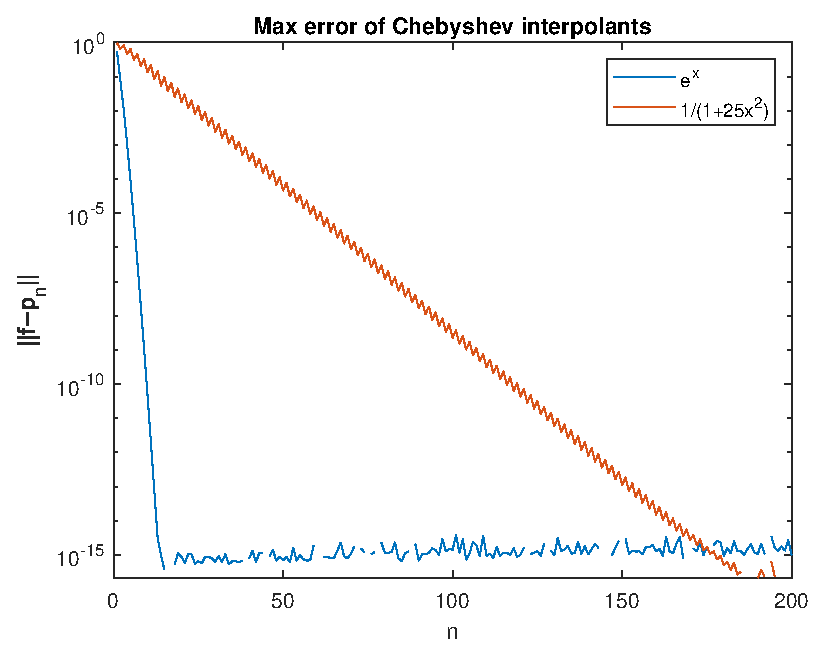
\includegraphics[]{prob2-5.eps}\\
For $f(x) = e^x$, we quickly reach machine precision at around $n=15$. After this, the error bounces around machine precision and is sometimes returned as identically zero. For Runge's function, convergence is much slower, reaching machine precision around $n=182$. After this, it experiences very similar behavior, bouncing around machine precision and registering the error as being identically zero. The convergence pattern is also interesting, because the error seems to increase every other iteration.   \\
See problem2\_5.m for the code that produces this plot.
\subsection{Exercise 3.2}
Using chebfun to compute numerically the coefficient of $T_5$ in the Chebyshev expansion of $\tan^{-1}(x)$ on $[-1,1]$, we get that it is about $4.877324*10^{-3}$.\\
See problem3\_2.m for the code that does this.
\subsection{Exercise 3.6}
\subsubsection{Part a}
We wish to derive the Chebyshev series coefficients for the function $f(x)=\sign(x)$ which are given by
\[
a_k=\frac{1}{2\pi i}\int_{|z|=1}(z^{-1+k}+z^{-1-k})\sign(\frac{z+z^{-1}}{2})dz
\]
Parameterize this as $z=e^{i\theta}$ and note that the $2\pi$-periodicity of these functions allows us to shift the bounds of integration
\[
a_k=\frac{1}{2\pi i}\int_{-\pi/2}^{3\pi/2}e^{-i\theta}(e^{ik\theta}+e^{-ik\theta})\sign(\cos\theta)(ie^{i\theta}d\theta)=\frac{1}{2\pi}\int_{-\pi/2}^{3\pi/2}(e^{ik\theta}+e^{-ik\theta})\sign(\cos\theta)d\theta.
\]
Now, note that $\cos\theta$ is positive on $(-\pi/2,\pi/2)$ and negative on $(\pi/2,3\pi/2)$ and that $(e^{ik\theta}+e^{-ik\theta})=2\cos(k\theta)$ by the definition of the complex cosine. Then,
\[
\begin{split}
a_k&=\frac{1}{\pi}\bigg(\int_{-\pi/2}^{\pi/2}\cos(k\theta)d\theta-\int_{\pi/2}^{3\pi/2}\cos(k\theta)d\theta\bigg)=\frac{1}{\pi}\bigg(\left[\frac{\sin(k\theta)}{k}\right]_{-\pi/2}^{\pi/2}-\left[\frac{\sin(k\theta)}{k}\right]_{\pi/2}^{2\pi/2}\bigg)\\&=
\frac{1}{\pi k}\bigg(\sin(\frac{k\pi}{2})-\sin(\frac{-k\pi}{2})-\sin(\frac{3k\pi}{2})+\sin(\frac{k\pi}{2})\bigg)
\end{split}
\]
Note that $\sin(\frac{3k\pi}{2})=\sin(\frac{-k\pi}{2})$ when $k\in\mathbb{Z}$ and that sine is an odd function. Then, 
\[
a_k=\frac{1}{\pi k}\bigg(2\sin(\frac{k\pi}{2})-2\sin(\frac{-k\pi}{2})\bigg)=\frac{4}{\pi k}\sin(\frac{k\pi}{2}).
\]
This expression is 0 if $k$ is even and $\frac{4}{\pi k}(-1)^{(k-1)/2}$ if $k$ is odd.
\subsection{Exercise 3.9}
We wish to show that derivatives of the Chebyshev polynomials satisfy $T'_n(1)=n^2$ for each $n\geq0$; we do so by strong induction on $n$. For a base case, note that $T_0(x)=1$ and $T_1(x)=x$, so $T'_0(1)=0=0^2$ and $T'_1(1)=1=1^2$. Now, say that $T'_n(1)=n^2$ for any $0\leq n\leq k$; we wish to show that $T'_{k+1}(1)=(k+1)^2$. From the recurrence relation of the Chebyshev polynomials, we have that $T_{k+1}(x)=2xT_k(x)-T_{k-1}(x)$. Thus,
$T'_{k+1}(x)=2T_k(x)+2xT'_k(x)-T'_{k-1}(x)$ and
\[
T'_{k+1}(1)=2T_k(1)+2xT'_k(1)-T'_{k-1}(1)=2*1+2*1*k^2-(k-1)^2=k^2+2k+1=(k+1)^2.
\]
Note that we have used the fact that $T_n(1)=1$ for any $n$. Thus, the inductive hypothesis holds for the $(k+1)$th case, meaning that $T'_n(1)=n^2$ for each $n\geq0$ holds by induction.

\subsection{Exercise 4.1}
Consider the polynomial $p(x)=2^{-n}(T_{n+1}(x)-T_{n-1}(x))$ and take $m=n-1<n$. Then, Theorem 4.1 gives that $T_m=T_{n-1}$ and $T_{2n-m}=T_{n+1}$ take the same values on an $(n+1)$-point Chebyshev grid. Thus, $p(x)$ has zeroes at the $n+1$ Chebyshev points. From page 15 of ATAP, we have that $T_{n+1}$ has leading coefficient $2^n$, so $p(x)$ must be a monic polynomial in $\mathcal{P}_{n+1}$, because $T_{n+1}\in\mathcal{P}_{n+1}$ and $T_{n-1}\in\mathcal{P}_{n-1}$. To show uniqueness, consider another polynomial $q(x)$ that is monic and has zeroes at the $n+1$ Chebyshev points. Then, the polynomial $p(x)-q(x)\in\mathcal{P}_n$ also has zeroes at the $n+1$ Chebyshev points. However, because it is a polynomial of degree $n$, this can only be true if $p(x)-q(x)=0$ identically.
\end{document}
